\documentclass{standalone}
\usepackage{tikz}
\usetikzlibrary{patterns, positioning}

\begin{document}
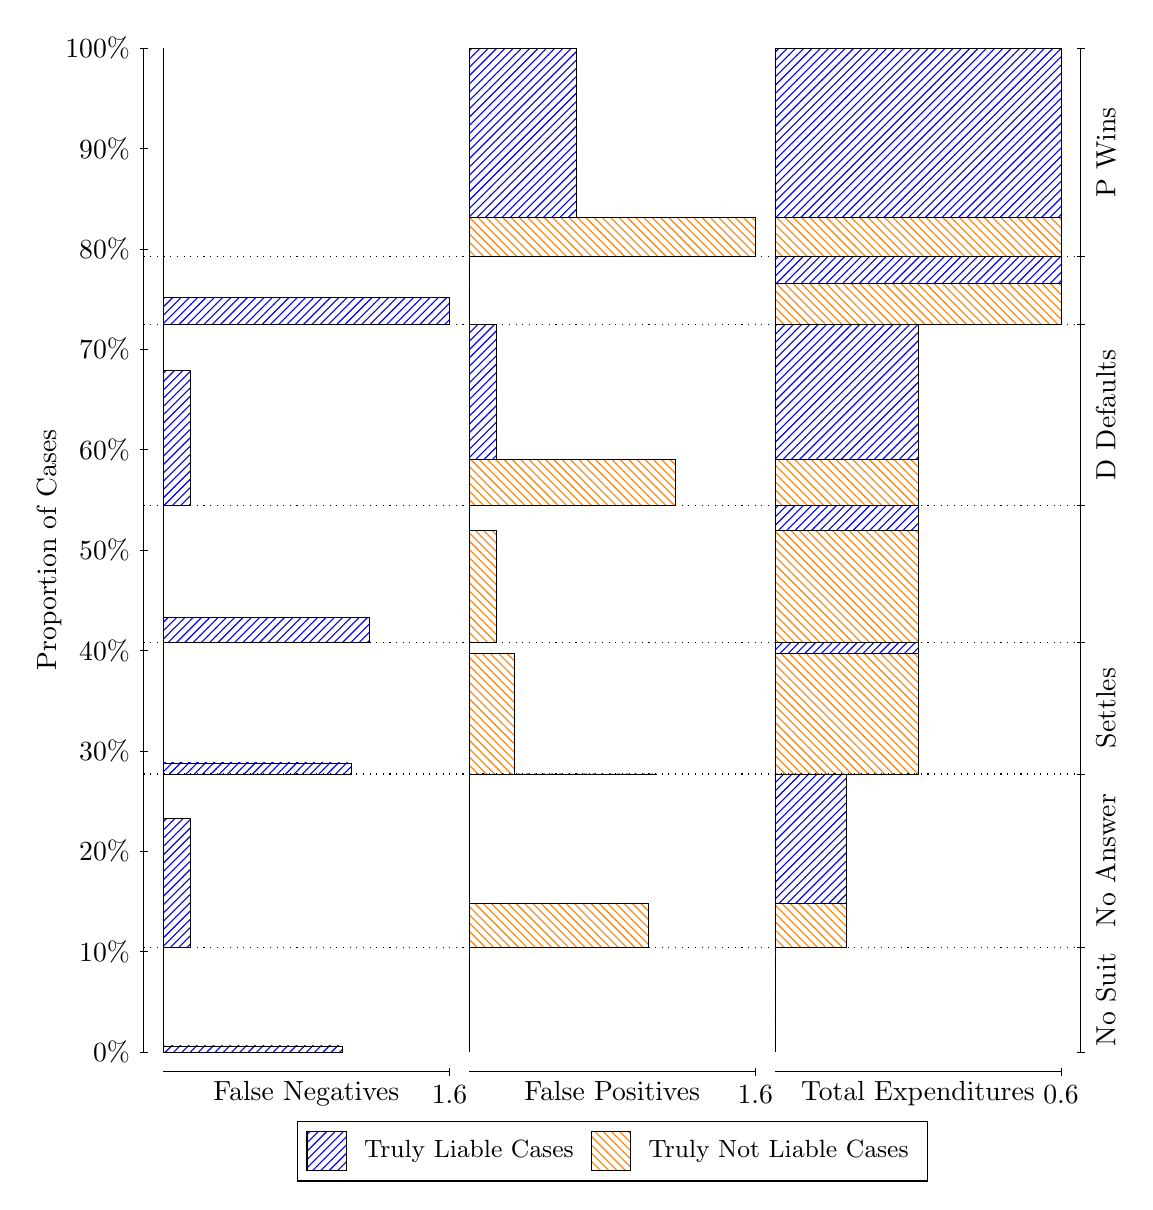
\begin{tikzpicture}
\draw[black, very thin] (1.5,1.75) -- (1.5,14.5);
\node[rotate=90, anchor=center] at (0.3, 8.125) {Proportion of Cases};
\draw[black, very thin] (1.45,1.75) -- (1.55,1.75);
\node[anchor=east] at (1.45, 1.75) {0\%};
\draw[black, very thin] (1.45,3.025) -- (1.55,3.025);
\node[anchor=east] at (1.45, 3.025) {10\%};
\draw[black, very thin] (1.45,4.3) -- (1.55,4.3);
\node[anchor=east] at (1.45, 4.3) {20\%};
\draw[black, very thin] (1.45,5.575) -- (1.55,5.575);
\node[anchor=east] at (1.45, 5.575) {30\%};
\draw[black, very thin] (1.45,6.85) -- (1.55,6.85);
\node[anchor=east] at (1.45, 6.85) {40\%};
\draw[black, very thin] (1.45,8.125) -- (1.55,8.125);
\node[anchor=east] at (1.45, 8.125) {50\%};
\draw[black, very thin] (1.45,9.4) -- (1.55,9.4);
\node[anchor=east] at (1.45, 9.4) {60\%};
\draw[black, very thin] (1.45,10.675) -- (1.55,10.675);
\node[anchor=east] at (1.45, 10.675) {70\%};
\draw[black, very thin] (1.45,11.95) -- (1.55,11.95);
\node[anchor=east] at (1.45, 11.95) {80\%};
\draw[black, very thin] (1.45,13.225) -- (1.55,13.225);
\node[anchor=east] at (1.45, 13.225) {90\%};
\draw[black, very thin] (1.45,14.5) -- (1.55,14.5);
\node[anchor=east] at (1.45, 14.5) {100\%};

\draw[black, very thin] (13.4,1.75) -- (13.4,14.5);
\draw[black, very thin] (13.35,1.75) -- (13.45,1.75);
\node[anchor=west] at (13.35, 1.75) {};
\draw[black, very thin] (13.35,3.0775) -- (13.45,3.0775);
\node[anchor=west] at (13.35, 3.0775) {};
\draw[black, very thin] (13.35,5.2807) -- (13.45,5.2807);
\node[anchor=west] at (13.35, 5.2807) {};
\draw[black, very thin] (13.35,6.9545) -- (13.45,6.9545);
\node[anchor=west] at (13.35, 6.9545) {};
\draw[black, very thin] (13.35,8.6868) -- (13.45,8.6868);
\node[anchor=west] at (13.35, 8.6868) {};
\draw[black, very thin] (13.35,10.992) -- (13.45,10.992);
\node[anchor=west] at (13.35, 10.992) {};
\draw[black, very thin] (13.35,11.849) -- (13.45,11.849);
\node[anchor=west] at (13.35, 11.849) {};
\draw[black, very thin] (13.35,14.5) -- (13.45,14.5);
\node[anchor=west] at (13.35, 14.5) {};

\draw[black, very thin, pattern color=blue, pattern=north east lines] (1.75,1.75) rectangle (4.0208,1.8278);
\draw[black, very thin, pattern color=orange, pattern=north west lines] (1.75,1.8278) rectangle (1.75,3.0775);
\draw[black, very thin, pattern color=blue, pattern=north east lines] (1.75,3.0775) rectangle (2.0906,4.7192);
\draw[black, very thin, pattern color=orange, pattern=north west lines] (1.75,4.7192) rectangle (1.75,5.2807);
\draw[black, very thin, pattern color=blue, pattern=north east lines] (1.75,5.2807) rectangle (4.1344,5.4216);
\draw[black, very thin, pattern color=blue, pattern=north east lines] (1.75,5.4216) rectangle (3.9073,5.4216);
\draw[black, very thin, pattern color=blue, pattern=north east lines] (1.75,5.4216) rectangle (3.6802,5.4216);
\draw[black, very thin, pattern color=blue, pattern=north east lines] (1.75,5.4216) rectangle (3.4531,5.4216);
\draw[black, very thin, pattern color=blue, pattern=north east lines] (1.75,5.4216) rectangle (3.226,5.4216);
\draw[black, very thin, pattern color=blue, pattern=north east lines] (1.75,5.4216) rectangle (2.999,5.4216);
\draw[black, very thin, pattern color=blue, pattern=north east lines] (1.75,5.4216) rectangle (2.7719,5.4216);
\draw[black, very thin, pattern color=blue, pattern=north east lines] (1.75,5.4216) rectangle (2.5448,5.4216);
\draw[black, very thin, pattern color=blue, pattern=north east lines] (1.75,5.4216) rectangle (2.3177,5.4216);
\draw[black, very thin, pattern color=orange, pattern=north west lines] (1.75,5.4216) rectangle (1.75,6.9545);
\draw[black, very thin, pattern color=blue, pattern=north east lines] (1.75,6.9545) rectangle (4.3615,7.2644);
\draw[black, very thin, pattern color=orange, pattern=north west lines] (1.75,7.2644) rectangle (1.75,8.6868);
\draw[black, very thin, pattern color=blue, pattern=north east lines] (1.75,8.6868) rectangle (2.0906,10.404);
\draw[black, very thin, pattern color=orange, pattern=north west lines] (1.75,10.404) rectangle (1.75,10.992);
\draw[black, very thin, pattern color=blue, pattern=north east lines] (1.75,10.992) rectangle (5.3833,11.331);
\draw[black, very thin, pattern color=orange, pattern=north west lines] (1.75,11.331) rectangle (1.75,11.849);
\draw[black, very thin, pattern color=orange, pattern=north west lines] (1.75,11.849) rectangle (1.75,12.352);
\draw[black, very thin, pattern color=blue, pattern=north east lines] (1.75,12.352) rectangle (1.75,14.5);
\draw[black, very thin, pattern color=orange, pattern=north west lines] (5.6333,1.75) rectangle (5.6333,2.9997);
\draw[black, very thin, pattern color=blue, pattern=north east lines] (5.6333,2.9997) rectangle (5.6333,3.0775);
\draw[black, very thin, pattern color=orange, pattern=north west lines] (5.6333,3.0775) rectangle (7.9042,3.6389);
\draw[black, very thin, pattern color=blue, pattern=north east lines] (5.6333,3.6389) rectangle (5.6333,5.2807);
\draw[black, very thin, pattern color=orange, pattern=north west lines] (5.6333,5.2807) rectangle (8.0177,5.2807);
\draw[black, very thin, pattern color=orange, pattern=north west lines] (5.6333,5.2807) rectangle (7.7906,5.2807);
\draw[black, very thin, pattern color=orange, pattern=north west lines] (5.6333,5.2807) rectangle (7.5635,5.2807);
\draw[black, very thin, pattern color=orange, pattern=north west lines] (5.6333,5.2807) rectangle (7.3365,5.2807);
\draw[black, very thin, pattern color=orange, pattern=north west lines] (5.6333,5.2807) rectangle (7.1094,5.2807);
\draw[black, very thin, pattern color=orange, pattern=north west lines] (5.6333,5.2807) rectangle (6.8823,5.2807);
\draw[black, very thin, pattern color=orange, pattern=north west lines] (5.6333,5.2807) rectangle (6.8823,5.2807);
\draw[black, very thin, pattern color=orange, pattern=north west lines] (5.6333,5.2807) rectangle (6.6552,5.2807);
\draw[black, very thin, pattern color=orange, pattern=north west lines] (5.6333,5.2807) rectangle (6.4281,5.2807);
\draw[black, very thin, pattern color=orange, pattern=north west lines] (5.6333,5.2807) rectangle (6.201,6.8136);
\draw[black, very thin, pattern color=blue, pattern=north east lines] (5.6333,6.8136) rectangle (5.7469,6.8136);
\draw[black, very thin, pattern color=blue, pattern=north east lines] (5.6333,6.8136) rectangle (5.6333,6.9545);
\draw[black, very thin, pattern color=orange, pattern=north west lines] (5.6333,6.9545) rectangle (5.974,8.3769);
\draw[black, very thin, pattern color=blue, pattern=north east lines] (5.6333,8.3769) rectangle (5.6333,8.6868);
\draw[black, very thin, pattern color=orange, pattern=north west lines] (5.6333,8.6868) rectangle (8.2448,9.2745);
\draw[black, very thin, pattern color=blue, pattern=north east lines] (5.6333,9.2745) rectangle (5.974,10.992);
\draw[black, very thin, pattern color=orange, pattern=north west lines] (5.6333,10.992) rectangle (5.6333,11.509);
\draw[black, very thin, pattern color=blue, pattern=north east lines] (5.6333,11.509) rectangle (5.6333,11.849);
\draw[black, very thin, pattern color=orange, pattern=north west lines] (5.6333,11.849) rectangle (9.2667,12.352);
\draw[black, very thin, pattern color=blue, pattern=north east lines] (5.6333,12.352) rectangle (6.9958,14.5);
\draw[black, very thin, pattern color=orange, pattern=north west lines] (9.5167,1.75) rectangle (9.5167,2.9997);
\draw[black, very thin, pattern color=blue, pattern=north east lines] (9.5167,2.9997) rectangle (9.5167,3.0775);
\draw[black, very thin, pattern color=orange, pattern=north west lines] (9.5167,3.0775) rectangle (10.425,3.6389);
\draw[black, very thin, pattern color=blue, pattern=north east lines] (9.5167,3.6389) rectangle (10.425,5.2807);
\draw[black, very thin, pattern color=orange, pattern=north west lines] (9.5167,5.2807) rectangle (11.333,5.2807);
\draw[black, very thin, pattern color=blue, pattern=north east lines] (9.5167,5.2807) rectangle (11.333,5.2807);
\draw[black, very thin, pattern color=orange, pattern=north west lines] (9.5167,5.2807) rectangle (11.333,6.8136);
\draw[black, very thin, pattern color=blue, pattern=north east lines] (9.5167,6.8136) rectangle (11.333,6.9545);
\draw[black, very thin, pattern color=orange, pattern=north west lines] (9.5167,6.9545) rectangle (11.333,6.9545);
\draw[black, very thin, pattern color=blue, pattern=north east lines] (9.5167,6.9545) rectangle (11.333,6.9545);
\draw[black, very thin, pattern color=orange, pattern=north west lines] (9.5167,6.9545) rectangle (11.333,8.3769);
\draw[black, very thin, pattern color=blue, pattern=north east lines] (9.5167,8.3769) rectangle (11.333,8.6868);
\draw[black, very thin, pattern color=orange, pattern=north west lines] (9.5167,8.6868) rectangle (11.333,9.2745);
\draw[black, very thin, pattern color=blue, pattern=north east lines] (9.5167,9.2745) rectangle (11.333,10.992);
\draw[black, very thin, pattern color=orange, pattern=north west lines] (9.5167,10.992) rectangle (13.15,11.509);
\draw[black, very thin, pattern color=blue, pattern=north east lines] (9.5167,11.509) rectangle (13.15,11.849);
\draw[black, very thin, pattern color=orange, pattern=north west lines] (9.5167,11.849) rectangle (13.15,12.352);
\draw[black, very thin, pattern color=blue, pattern=north east lines] (9.5167,12.352) rectangle (13.15,14.5);
\draw[black, dotted] (1.5,3.0775) -- (13.4,3.0775);
\draw[black, dotted] (1.5,5.2807) -- (13.4,5.2807);
\draw[black, dotted] (1.5,6.9545) -- (13.4,6.9545);
\draw[black, dotted] (1.5,8.6868) -- (13.4,8.6868);
\draw[black, dotted] (1.5,10.992) -- (13.4,10.992);
\draw[black, dotted] (1.5,11.849) -- (13.4,11.849);
\draw[black, very thin] (1.75,1.5) -- (5.3833,1.5);
\node[anchor=north] at (3.5667, 1.5) {False Negatives};
\draw[black, very thin] (5.3833,1.45) -- (5.3833,1.55);
\node[anchor=north] at (5.3833, 1.45) {1.6};

\draw[black, very thin] (5.6333,1.5) -- (9.2667,1.5);
\node[anchor=north] at (7.45, 1.5) {False Positives};
\draw[black, very thin] (9.2667,1.45) -- (9.2667,1.55);
\node[anchor=north] at (9.2667, 1.45) {1.6};

\draw[black, very thin] (9.5167,1.5) -- (13.15,1.5);
\node[anchor=north] at (11.333, 1.5) {Total Expenditures};
\draw[black, very thin] (13.15,1.45) -- (13.15,1.55);
\node[anchor=north] at (13.15, 1.45) {0.6};

\node[black, centered, rotate=90] at (13.72, 2.4137) {No Suit};
\node[black, centered, rotate=90] at (13.72, 4.1791) {No Answer};
\node[black, centered, rotate=90] at (13.72, 6.1176) {Settles};

\node[black, centered, rotate=90] at (13.72, 9.8392) {D Defaults};

\node[black, centered, rotate=90] at (13.72, 13.174) {P Wins};

\draw (7.449999999999999,1.5) node[draw=none] (baseCoordinate) {};
\begin{scope}[align=center]
        \matrix[scale=0.5, draw=black, below=0.5cm of baseCoordinate, nodes={draw}, column sep=0.1cm]{
            \node[rectangle, draw, minimum width=0.5cm, minimum height=0.5cm, pattern=north east lines, pattern color=blue] {}; &
            \node[draw=none, font=\small] (B) {Truly Liable Cases}; &
            \node[rectangle, draw, minimum width=0.5cm, minimum height=0.5cm, pattern=north west lines, pattern color=orange] {}; &
            \node[draw=none, font=\small] (B) {Truly Not Liable Cases}; \\
            };
\end{scope}

\end{tikzpicture}
\end{document}